\chapter{Opdracht 3: Application service}
We hebben het project aan de praat, de eisen geanalyseerd, 
de use cases gemodelleerd en de eerste domeinconcepten gerealiseerd. 
Het doet allemaal alleen nog niet zoveel!

\section{Spring Boot}
Spring Boot is een veelgebruikte standaardconfiguratie van het Spring framework. 
Vanaf gaan we ons mooie java-domein-model aanspreken met een echte Webservice.

In deze fase gebruiken we al wel de HTTP-functionaliteit van Spring (@RestControllers), maar
de database is er nog niet. Daarvoor gebruiken we een In-memory nep-implementatie. Voorlopig 
zal dus alle data ge-reset zijn elke keer dat je de applicatie opnieuw opstart (maar geen zorgen
dat pakken we later weer op!).

\subsection{Project Structuur}

Ondertussen is de mappen- en packagestructuur onder \texttt{src/main/java} een stuk uitgebreider geworden:

\dirtree{%
    .1 nl.hu.bep2.casino.
        .2 chips.
            .3 presentation.
                .4 controller.
                .4 dto.
            .3 application.
            .3 domain.
                .4 exception.
            .3 data.
        .2 security.
        .2 blackjack.
            .3 (...).
}

Het project is dus eerst opgedeeld in verschillende componenten en vervolgens in 
lagen. In lagen kunnen we zaken weer groeperen in deelsystemen. Deze componenten 
en lagen kunnen we weergeven als packages, zie Figuur~\ref{fig:uml-casino-physical-layers}.

\begin{figure}[H]
    \centering
    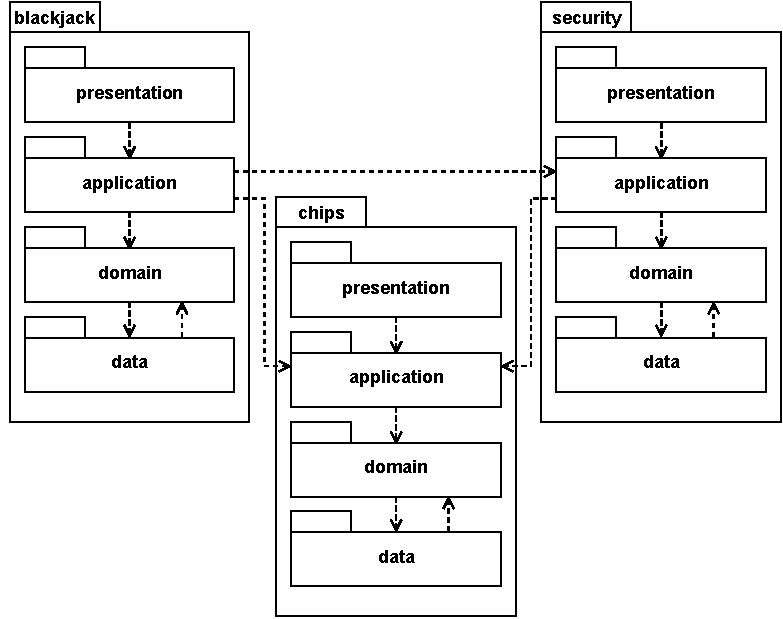
\includegraphics[width=.6\linewidth]{uml-casino-physical-layers}
    \caption{Components en layers kunnen met packages worden aangewezen binnen het casinoproject.}
    \label{fig:uml-casino-physical-layers}
\end{figure}

\subsubsection{Componenten}
Een component is een opzichzelfstaand onderdeel van een softwaresysteem
dat ziet op een bepaald deelgebied aan functionaliteit, bijvoorbeeld op een 
bepaald subdomein.

Het component bevat een aantal domeinobjecten. 
De communicatie wordt aangeboden via een service (ook: \textit{facade}). 
Deze service kan worden aangesproken door andere
services, maar ook door bijvoorbeeld een controller of een commando uit een commandline interface. 
De controller is bedoeld om HTTP-communicatie om te zetten naar Java code en vice versa. 
Andersom praat het component alleen met de buitenwereld, zoals een database, via een \textit{gateway}.

In ons project maken we gebruik van Spring om controllers te schrijven.
Deze controllers kunnen dan door Spring worden aangeroepen 
wanneer een bepaald web request moet worden afgehandeld.
Aan de andere kant maken we later ook gebruik van Spring om te voorzien in 
de data-opslag aan de hand van repositories.

\subsubsection{Lagen}
Een applicatie, of een deel ervan, is vaak opgedeeld in lagen die 
elk verantwoordelijk zijn voor een ander soort logica binnen het systeem.
Het afhandelen van gebruikersinteractie 
is bijvoorbeeld iets heel anders dan het uitdelen van kaarten in een
kaartspel of het opslaan van een speelronde.
Een gelaagde structuur helpt niet alleen met het terugvinden van
bepaalde klassen op basis van het soort logica dat het betreft. Bij een 
losgekoppeld ontwerp kunnen lagen of onderdelen ervan gemakkelijk uitgewisseld worden.

Gelaagde architecturen komen in verschillende soorten en maten. Sommige applicaties 
zijn eerst opgesplitst in componenten en vervolgens ingedeeld in lagen. Andere zijn 
eerst opgesplitst in lagen, waarin vervolgens losse componenten zijn te bespeuren.
Het aantal lagen kan variëren tussen de twee en vijf lagen. Dit hangt af 
van de verschillende soorten logica en de specifieke architecturele eisen
van de onderdelen binnen een project.

Deze packages corresponderen met de volgende soorten logica:
\begin{itemize}
    \item \emph{Presentation}: Presentatielogica. In het geval van een back-end API tref
    je hier alles aan dat hoort bij de technische vertaling van web requests naar Java-code. 
    Controllers (web request handlers) worden aangeroepen door het Spring framework 
    zodra een HTTP-request binnenkomt met een gedefinieerde route (HTTP-method + URL).
    \item \emph{Application}: Taakspecifieke logica. Hierin zitten applicatieservices (\emph{facades}) 
    die use cases omzetten naar domeinacties met behulp van infrastructuurabstracties. Een applicatieservice
    ziet vaak op één centraal domeinobject dat is opgebouwd uit of verwijst naar andere domeinobjecten.
    Door een applicatielaag in te richten kan dezelfde logica geboden worden onafhankelijk van de gebruikte 
    technologie in de presentatielaag: command line commando's, GUI's, web controllers of message handlers.
    \item \emph{Domain}: Domeinlogica. Domeinconcepten, business rules en entiteiten vind je vaak in lagen 
    met deze verantwoordelijkheid.
    \item \emph{Data}: Infrastructuurabstractie. Hierin zitten meestal interfaces of abstracte klassen die door
    infrastructuurklassen moeten worden ingevuld (\emph{gateways}).
\end{itemize}

Probeer voor jezelf de volgende vragen te beantwoorden, eventueel door naar de code te kijken.
Welke klasse is verantwoordelijk voor de vertaling van HTTP-verkeer naar Java en andersom?
In welke klassen zal je de use cases van dit component terugzien?
In welke methode wordt het aantal chips verminderd bij een afschrijving?
Hoe denk je dat de opslag geregeld is?
Stel een ander component binnen ons systeem wil Chips opnemen voor een user, welke klasse wordt dan 
eerst aangesproken?

Je mag dit met docenten en medestudenten overleggen, 
maar het antwoord op deze vragen zal naar verloop van tijd duidelijker worden.

\subsubsection*{Kanttekening: Geen écht lagenmodel}
Het casinoproject is opgezet met de verschillende soorten logica in gedachten. 
Als je het lagenmodel echter strikt zou toepassen op Figuur~\ref{fig:uml-casino-physical-layers}, 
zie je een overtreding in de laatste twee lagen van elk component. 
Hier gaan we later in dit collegejaar op in (bij de cursus \textbf{Software Architecture}),
maar misschien wil je hier al wat meer over weten.

De datalaag bestaat weliswaar slechts uit interfaces die door 
Spring geïmplementeerd worden, maar ze zijn afhankelijk van objecten (entiteiten) die
gedefinieerd zijn in het domein. Logisch gezien zou je het project daarom 
eerder beschouwen als een drie-lagen-architectuur! De laatste laag zou dan 
conceptueel zowel domeinlogica als infrastructuurabstracties bevatten. 
Deze laag is dan fysiek (in onze code) opgedeeld in twee Java packages 
om de abstracte, stabiele kern (domein) te scheiden van de meer flexibele 
aansluiting met infrastructuur via interfaces (data). 
Het casino-project kent verder een flexible layered architecture: 
je mag lagen overslaan.
Zo mag je in de presentatielaag een domeinobject teruggeven,
zodat het in een HTTP-response kan worden opgenomen, en exceptions uit het domein 
afhandelen zodat een HTTP-response de juiste statuscode kan hebben.
Dit is in veel gelaagde architecturen niet het geval. In die architecturen 
heeft een laag alleen koppeling met de laag rechtstreeks eronder.
In ons project is dit niet nodig. Het scheelt een hoop extra code en we 
tolereren de extra koppeling.

\begin{figure}[H]
    \centering
    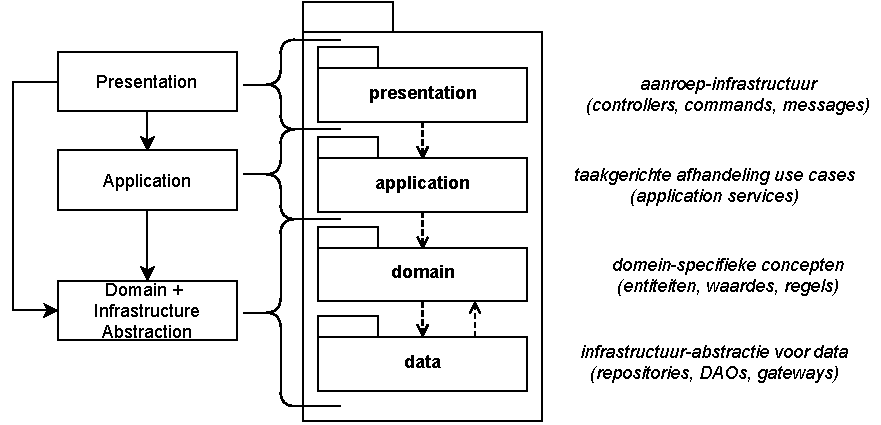
\includegraphics[width=.7\linewidth]{casino-layers}
    \caption{Het logisch en fysiek lagenmodel binnen het componenten van het casinoproject.}
    \label{fig:casino-layers}
\end{figure}

Als je de realisatie toch meer wil afstemmen op de laging, zou je de 
data-objecten en domein-objecten van elkaar splitsen en deze als losse objecten opnemen in de datalaag.
Daarvoor moet je dan daartussen een vertaalslag aanbieden. 
Als je daarnaast wil verbieden dat er lagen worden overgeslagen, 
zou je ook een vertaalslag kunnen toevoegen tussen domeinobjecten en presentatie-objecten.
Als alternatief zou je de infrastructuur-abstractie
(de repositories) kunnen opnemen in het domein en dat \textit{data} package verwijderen.
In ons project passen we deze regels echter niet zo strikt toe:
we accepteren een lichte koppeling op het framework en op ons domein.

\subsubsection{Subsystems}
Een laag kan nog verder worden opgebroken in subsystems (of \textit{deelsystemen}).
Dit zijn algemene packages die zijn bedoeld om een reeks objecten samen te verpakken.

\subsection{Voorbeeld: Structuur binnen het chips-component}
Elk component is in lagen opgedeeld. In het chips-component ziet 
dat eruit zoals in Figuur~\ref{fig:chips-layers}.

\begin{figure}[H]
    \centering
    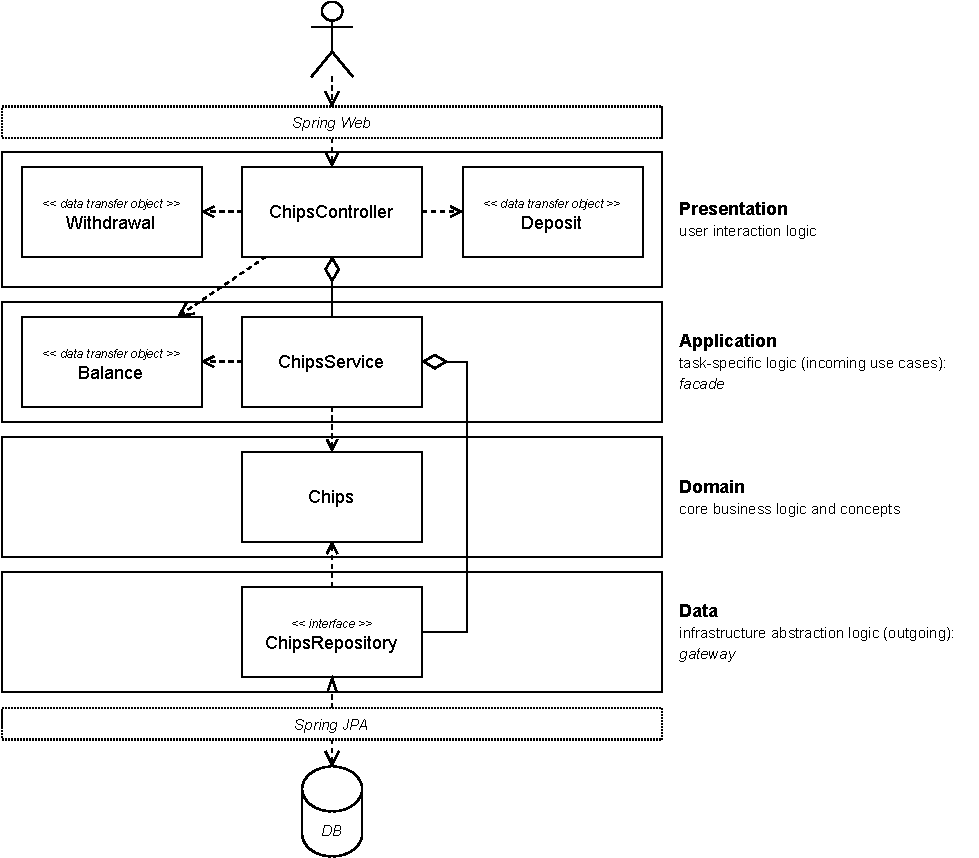
\includegraphics[width=0.8\linewidth]{chips-layers}
    \caption{De semi-gelaagde structuur binnen het chips-component.}
    \label{fig:chips-layers}
\end{figure}

\subsection{Applicatieflow}
Hoe loopt de flow binnen de de lagen in een component? 
Laten we daarvoor een blik werpen 
op de \emph{deposit use case} van het Chips-component.
Zie Figuur~\ref{fig:chips-sequence-diagram}.

\begin{figure}[H]
    \centering
    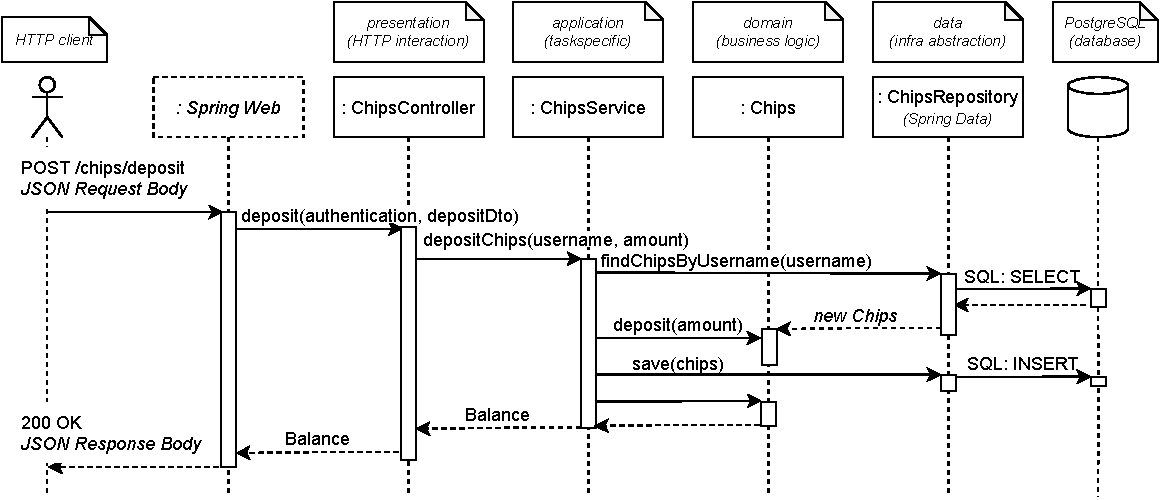
\includegraphics[width=\linewidth]{chips-sequence-diagram}
    \caption{De flow voor de deposit use case van het Chips-component}
    \label{fig:chips-sequence-diagram}
\end{figure}

Kijk ook in de code of je dit kunt herkennen!
Allereerst moet een HTTP-client een POST-verzoek doen naar 
\texttt{/chips/deposit}. We willen namelijk een overmaking toevoegen
aan de chips resource voor de huidige gebruiker. In dat POST-verzoek 
wordt de huidige gebruiker meegegeven via een JWT-token in de Authorization header
als deze is ingelogd. 

Vervolgens zet Spring Web dit verzoek om naar de bijbehorende 
controlleractie op de \emph{ChipsController} in de presentatielaag, met de
nodige informatie over de gebruiker (\emph{Authentication}) en de data die 
in de HTTP JSON Request Body zit (het \emph{Deposit} data transfer object).
De controller haalt de nodige data uit deze objecten en zet dit om naar 
een aanroep op de \emph{ChipsService} in de applicatielaag. 
Deze ChipsService bevat allerlei methoden die de use cases van 
het Chips-component vertegenwoordigen.
De service roept de \emph{ChipsRepository} aan uit de datalaag om de hoeveelheid
\emph{Chips} op te vragen voor de betreffende \emph{User} (op basis van de username). 
Vervolgens roept de service de \emph{deposit}-methode aan op de Chips om het aantal chips te verhogen met de 
gekozen hoeveelheid en wordt het \emph{Chips} object weer opgeslagen in de \emph{ChipsRepository}.
Ten slotte geeft de service een \emph{Balance} terug door de benodigde data uit het 
\emph{Chips}-object te halen en dit in een nieuw \emph{Balance}-object te stoppen.
De controller geeft ook deze \emph{Balance} terug aan Spring Web, waarop deze de 
\emph{Balance} omzet naar een HTTP JSON Response Body aan de hand van diens getters.

Voor het blackjack-component zou het ideaal zijn als wij ook één centraal object hebben 
om op te halen, domeinacties op uit te voeren en weer weg te schrijven. Het aan elkaar 
knopen daarvan kan gebeuren in use cases aangeboden in een BlackjackService!

\subsection{Frameworks}
Een \textit{framework} is code van anderen die je een hoop werk uit handen 
nemen ten aanzien van een of meer functionaliteiten. Het is een concrete, herbruikbare standaardoplossing.
Kenmerkend aan een framework is dat je als developer een deel van de controle 
uit handen geeft. Er is sprake van \textit{inversion of control}: het framework 
roept onze code aan op bepaalde plekken. Interactie met het framework vindt op twee plaatsen 
plaats:
\begin{enumerate}
    \item Entry points: hier roepen we het framework aan
    \item Hot spots: hier haken we onze eigen code in het framework en roept het framework onze code aan
\end{enumerate}

Er zijn twee soorten hot spots, die je kan herkennen vanuit het objectmodel:
\begin{enumerate}
    \item Composition hot spots: integratie van het aan een interface meegeven 
    van implementerende dependencies
    \item Inheritance hot spots: integratie via het overerven 
    van een vooropgezette klassenstructuur
\end{enumerate}

Beide vormen komen vaak voor in een framework.

In Spring herkennen we de \texttt{CasinoApplication} als entry point.
Deze is geannoteerd met \texttt{@SpringBootApplication}. Vervolgens laadt
Spring allerlei configuratie in, voert het een componentscan uit en klikt het dependencies in elkaar.
Spring's dependency injection is één van de composition hot spots die te vinden zijn in Spring,
terwijl Spring's repositories een vorm zijn inheritance hot spots.

\subsection{Dependency injection}
Dependency injection is niets anders dan het meegeven van afhankelijkheden,
in plaats van ze binnen de klasse aan te maken. Dit zorgt ervoor dat een klasse 
makkelijker uitbreidbaar en testbaar is. Hierover in een latere cursus meer.

In Spring maken we services aan door de klasse te annoteren met de \texttt{@Service} annotatie. 
We kunnen met dependency injection werken door de services (en opslagmechanismen) waarvan we afhankelijk zijn 
aan te geven in de constructor. Spring vindt dan automatisch welke services we bedoelen. 
Dit heet \textit{autowiring}.
Spring gaat tijdens een opstarten van de applicatie door onze code op zoek naar 
\texttt{@Bean}, \texttt{@Component}, \texttt{@Service}. Dit noem je Beans. 
Spring kijkt voor de dependencies naar de constructor en de benodigde interfaces 
en kijkt of er Beans zijn geconfigureerd die aan die interface voldoen. Met autowiring 
injecteert Spring de benodigde afhankelijkheid dus automatisch!

Kijk voor een voorbeeld wederom in het Chips-component.

Als alternatief voor constructor-injection kan 
je ook werken met de \texttt{@Autowired} annotatie 
op setters, constructor parameters of properties. 

Als we meerdere implementaties hebben van dezelfde interface 
(bijvoorbeeld omdat we een testimplementatie hebben), 
dan moeten we specifiek aangeven welke service we willen gebruiken. 
Dat kunnen we doen met de \texttt{@Qualifier} annotatie op zowel de service als binnen de constructor. 
Daarmee kwalificeren we om welke implementatieklasse het gaat door 
dit aan te geven boven elke \texttt{@Service} en vóór elke parameter in de 
constructor die de service gebruikt.

Met \texttt{@Value} kan je aangeven dat een waarde moet worden geïnjecteerd,
afkomstig is uit configuratie.

\section{Libraries}
Een library is ook een voorbeeld van een concrete, herbruikbare standaardoplossing.
Het belangrijkste verschil tussen een library en een framework is dat 
een framework veel meer controle opeist. Een library wordt door onze code aangeroepen
terwijl een framework uiteindelijk onze code aanroept (inversion of control).

Wel zie je vaak dat een framework gebruik maakt of zich openstelt voor verschillende
libraries door middel van composition hot spots. Vaak heb je dan een adapter nodig 
om de interface van het framework aan te passen aan de geboden facade van de library.
Dit zijn voorbeelden van design patterns. Hier gaan we het later uitgebreid over hebben.

\section{Stap 1: Maak een applicatieservice}
In ons domein hebben we een aantal domeinklassen gemaakt die verantwoordelijk 
zullen worden voor kleine acties per concept. Deze worden aan elkaar geknoopt 
door een dienstverlenend object dat verantwoordelijk is voor het omzetten van 
use cases naar domeinacties met behulp van infrastructuur. 
Dat wordt ook wel een \textit{application service} genoemd.

Maak eerst weer een package aan onder onze blackjack-component met de naam \texttt{application}
Dit is de applicatielaag waarin we onze taakgerichte logica (use cases) gaan uitvoeren.
Maak in die package een klasse aan: \texttt{BlackjackService}.
Het is immers een dienst die de acties aanbiedt om blackjack te kunnen spelen!
Deze wordt uiteindelijk aangesproken door de controller.

Vervolgens moeten we aan Spring doorgeven dat hij deze service kan gebruiken 
om te meegeven aan een andere service of bijvoorbeeld een controller als deze 
deze nodig heeft in de controller. Spring bevat een automatisch mechanisme 
voor \textit{dependency injection} en gebruikt daar annotaties voor. Om de service 
als zodanig vindbaar te maken, kan je \texttt{@Service} boven de klassedeclaratie plaatsen.

Dit zou er als volgt uit moeten zien:
\begin{minted}{java}
package nl.hu.bep2.casino.blackjack.application;

@Service
public class BlackjackService {
}
\end{minted}

\section{Stap 2: Bedenk welke methodes we nodig hebben}
Welke acties moet onze service aanbieden? 
Dit komt overeen met de use cases van onze component! 
Als het goed is, hebben we hiervoor een use case diagram gemaakt.

Maak public methods aan met de namen van deze use cases volgens 
de naming conventions van Java (\textit{camelCase}). 
Bedenk per methode ook wat voor een input we nodig hebben.
Voor sommige methoden is het handig om het spel te kunnen identificeren
op basis van een id (type: \textit{Long}). Voor de meeste methoden hebben 
we daarnaast de naam van de gebruiker nodig (type: \textit{String}).

De identifier zullen we automatisch door de database laten genereren
zodra we met persistentie bezig gaan.

\subsection{Voorbeeld: Het starten van het spel}
Laten we als voorbeeld het starten van een spel als use case nemen.
Het is belangrijk om hier een duidelijke, beschrijvende naam voor te pakken,
bijvoorbeeld: \textit{startGame} of \textit{start}.

\subsubsection{Method arguments}
Wat moeten we allemaal meegeven als parameters om het spel te starten?

Om het spel te kunnen opzoeken voor deze speler is het handig om de naam van de speler  
te bewaren. We kunnen een parameter toevoegen met als type \texttt{String} en 
als naam \texttt{playerName}. 
Omdat een speler meerdere spellen kan hebben, moeten we ervoor zorgen 
dat de database ook elk spel voorziet van een unieke identifier. 
Dat doen we later wanneer we met persistentie bezig gaan.

Het is handig om het spel meteen te beginnen met een inleg. Dat bespaart ons een
extra HTTP request! Laten we de parameter \texttt{Integer bet} toevoegen.

Meer hebben we niet nodig van de speler!

\subsubsection{Return type}
Wat willen we teruggeven nadat we het spel hebben gestart? 
Hier kunnen we wat slims verzinnen om aan de speler te laten zien hoe 
het spel er nu uitziet: de spelvoortgang. 
We willen uiteindelijk namelijk in de controller
een bericht terugsturen naar de HTTP client met daarin een JSON body 
met alle informatie. Een front-endprogrammeur kan dat mooi weergeven met
afbeeldingen en interacties.

Welke informatie willen we aan de speler laten zien
en hoe kunnen we dat het best structureren? Dat laten we aan jou over!
Alvast een tip: we kunnen een String teruggeven, 
maar dan gaat er een boel gestructureerde informatie verloren!

\subsection{Stap 3: Vul de methodes in}
Nadat we bedacht hebben welke methodes onze service moet hebben, 
kunnen we naar de invulling van die methodes kijken.
Het is het mooiste als applicatieservices niet teveel logica bevatten,
maar het gros van het werk door domeinobjecten wordt gedaan.
Op deze manier houd je een abstract en herbruikbaar domein en is je 
applicatieservice een soort samenvatting van hoe het domein zich gedraagt.

Probeer in algemene bewoordingen de acties te beschrijven 
en gaandeweg acties toe te voegen aan de centrale domeinentiteit
en de domeinobjecten die daarin gebruikt worden.

\subsubsection{Voorbeeld: Method body van startGame}
We hebben een methodenaam, parameters en een return type gedeclareerd.
Welke stappen willen we uitvoeren in de methode? 

Globaal zal je op de volgende zaken uitkomen:

\begin{enumerate}
    \item Neem het aantal chips op ter hoogte van de bet
    \item Maak een nieuw spel aan
    \item Start het spel
    \item Sla het spel op
    \item Stort chips als sprake van blackjack of push
    \item Geef de voortgang terug
\end{enumerate}

Voor het starten van het spel kan je een methode op het Game object maken,
genaamd \textit{start}. Je kan ervoor kiezen om de benodigde parameters mee te geven aan de 
constructor of de start methode. Wat deze methode moet doen laten we aan jou over.
Een aantal tips: wat moet de speltoestand zijn bij het beginnen van het spel?
Laat je het spel zelf een nieuwe Deck maken of doen we dat in de application service?

Bij de uitvoering van \textit{game.start()}, maken we onder andere gebruik van 
Deck en vast ook wel van andere klassen en enums! 
De kaarten moeten worden geschud en op de hand worden gebracht van de speler 
en van de dealer. Vervolgens moeten scores berekend worden en de huidige speltoestand 
geupdatet worden.

Het opslaan van het spel kan je nog even laten zitten,
maar het is misschien handiger om dit tijdelijk te doen 
door een field op te nemen in de application service.
Je zou hiervoor een \texttt{Map<String, Game>} kunnen gebruiken 
waarmee tijdelijk spellen (\textit{value}) bewaard kunnen worden 
op basis van spelernaam (\textit{key}).

Dit gaan we in een van de volgende opdrachten vervangen met apart object dat verantwoordelijk 
is voor de langdurige opslag van spellen: een GameRepository.

\subsubsection{Bescherm in domeinacties tegen ongeldige situaties (invariants)}
Je domein bepaalt hoe de regels van de kernconcepten eruit zien.
Bij een spel zijn het bijvoorbeeld letterlijk de spelregels.
Zie bijvoorbeeld de Chips-klasse: je mag geen negatieve hoeveelheid opnemen 
en je mag geen chips opnemen als je saldo te laag is.

\begin{minted}{java}
 public void withdraw(Long amountToWithdraw) {
    if (amountToWithdraw < 0) {
        throw new NegativeNumberException("Cannot withdraw a negative amount: " + amountToWithdraw);
    }

    long newAmount = this.amount - amountToWithdraw;
    if (newAmount < 0) {
        throw new NotEnoughChipsException(
                String.format(
                        "Cannot withdraw %d chips: %d chips remaining",
                        amountToWithdraw,
                        this.amount
                )
        );
    }

    this.amount = newAmount;
}    
\end{minted}

Voor het spelen van het spel geldt hetzelfde. Je mag natuurlijk 
geen zetten doen als het spel is afgelopen! Hiervoor kan je een \textit{guard-clause} gebruiken:
een \textit{if-statement} die een exception gooit als iets niet mag. Je hebt geen \textit{else} nodig! 
De flow wordt immers doorbroken als er sprake is van een exception.

\subsubsection{Overige use cases en domeinacties}
Doe hetzelfde voor de overige use cases en domeinacties. 
Hier gaat een boel tijd inzitten, 
dus het is niet erg als je dit later verbetert wanneer we 
de persistentie en de web API ingericht hebben.

Commit je wijzigingen met een duidelijke naam, 
bijvoorbeeld: "Add use cases to blackjack service". 
Push de wijzigingen naar je remote GitHub repository.